\documentclass{article}
\usepackage{tikz}
\usetikzlibrary{positioning}

\begin{document}

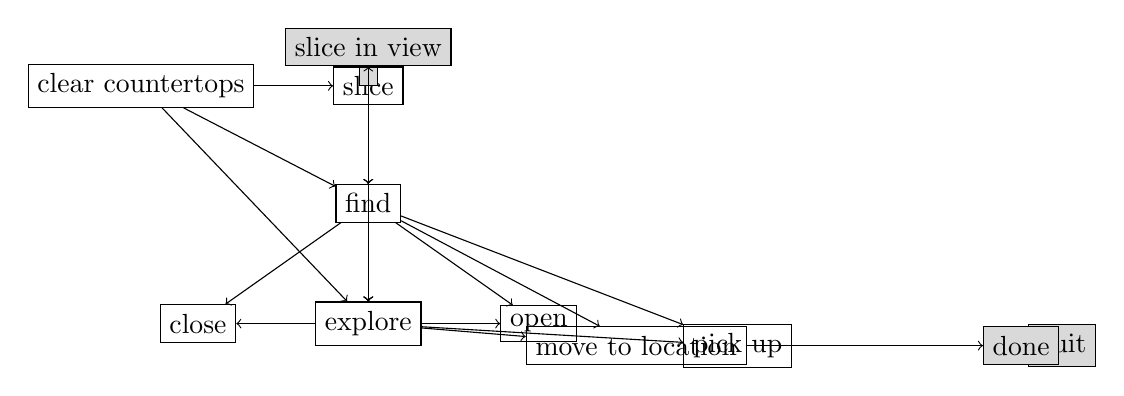
\begin{tikzpicture}[node distance=1cm, auto]
    \node [draw] (clear) {clear countertops};
    \node [draw, right=of clear] (slice) {slice};
    \node [draw, below=of slice] (find) {find};
    \node [draw, below=of find] (explore) {explore};
    \node [draw, below=of explore, left=of explore] (close) {close};
    \node [draw, below=of explore, right=of explore] (open) {open};
    \node [draw, below=of explore, right=2cm] (move) {move to location};
    \node [draw, below=of explore, right=4cm] (pick) {pick up};
    
    \path[->] 
        (clear) edge node {} (slice)
        (clear) edge node {} (find)
        (clear) edge node {} (explore)
        (slice) edge node {} (find)
        (slice) edge node {} (explore)
        (find) edge node {} (explore)
        (find) edge node {} (close)
        (find) edge node {} (open)
        (find) edge node {} (move)
        (find) edge node {} (pick)
        (explore) edge node {} (close)
        (explore) edge node {} (open)
        (explore) edge node {} (move)
        (explore) edge node {} (pick);
    
    \node [draw, fill=gray!30, above=of slice, yshift=-1cm] (view) {slice in view};
    \node [draw, fill=gray!30, below=of view, yshift=1cm] (in_view) {};
    
    \path[->] 
        (view) edge node {} (slice)
        (view) edge node {} (find)
        (view) edge node {} (explore)
        (in_view) edge node {} (find)
        (in_view) edge node {} (explore);
    
    \node [draw, fill=gray!30, right=of pick, xshift=2cm] (quit) {quit};
    
    \path[->] 
        (pick) edge node {} (quit);
    
    \node [draw, fill=gray!30, right=of move, xshift=2cm] (done) {done};
    
    \path[->] 
        (move) edge node {} (done);
\end{tikzpicture}

\end{document}